% !TeX encoding = UTF-8
% !TeX spellcheck = en_US
% !TeX root = ekg-mm/ekg-mm.tex
% !TEX program = lualatex
% !TEX options = -synctex=1 -interaction=nonstopmode -file-line-error "%DOC%"
% !BIB program = biber
% !BIB options = "%DOCFILE%" -bblencoding=utf8 -u -U --output_safechars "%DOCFILE%"
%
% The above are so called "magic comments" used by editors like TexStudio
%
\makeatletter\def\input@path{{../../../etc/}{../../etc/}{../etc/}}\makeatother
\documentclass{whitepaper-style-doc}

\loadGlossaries

\RequirePackage{maturity-model-stuff}

%
% The following two lines make sure that chapter numbers
% start with 1 within each part.
%
\RequirePackage{chngcntr}
\counterwithin*{chapter}{part}

\loadGlossaries

%
% Title page variables
%
\title{\glsfmtshort{ekgmm}}
\def\subtitleLineA{Overview of the Maturity Model}
\def\subtitleLineB{for the \glsxtrlong{ekg}}
\author{\agnos}
\date{\today}

\typeout{ekg-mm =================================> Start Document}
\begin{document}

\typeout{ekg-mm =================================> Intro}

\part{Intro}

\bgroup

\renewcommand{\thechapter}{\arabic{chapter}}
\renewcommand{\thesection}{\arabic{section}}
\renewcommand{\thesubsection}{\thesection.\arabic{subsection}}
\renewcommand{\thesubsubsection}{\thesubsection.\arabic{subsubsection}}

\section{Executive Summary}

\TODO[inline]{Write executive overview or summary before everything else so that we at least have something to explain this?}

\chapter{Strategy Objectives}
%
% TODO: Add all the concepts to the index
%
\begin{itemize}[leftmargin=2in,font=\bfseries]
  \item [Business Strategy] corporate objectives, use cases and organizational mechanisms necessary for sustainable business value from the \glsxtrfull{ekg}
  \begin{itemize}[labelwidth=1.5in,leftmargin=0in]
    \item [Corporate Goals] Alignment (shared vision) on why the organization is building a knowledge graph
    \item [Business Unit Goals] Support of the \glsxtrshort{ekg} value proposition\index{EKG Value Proposition} by key \glsxtrshort{lob} stakeholders\index{Stakeholders}
    \item [Organizational Considerations] Operational and resource plans for KG strategy implementation and governance
  \end{itemize}
  \item [Data Strategy] enterprise data management framework (policies, target data architecture, quality assurance, governance) necessary to support the knowledge graph environment
    \begin{itemize}[labelwidth=1.5in,leftmargin=0in]
      \item [Data Goals \& Objectives] Importance of unique identification and the value of unambiguous shared meaning
      \item [Knowledge Graph Positioning] Role of the \glsxtrshort{ekg} as the underlying data fabric for the organization
      \item [Business Case] ROI of linked data as an essential component of operational infrastructure
    \end{itemize}
  \item [Technology Strategy] environment for successful knowledge graph implementation including direction for physical infrastructure, applications and process automation
    \begin{itemize}[labelwidth=1.5in,leftmargin=0in]
      \item [Infrastructure Strategy] Physical infrastructure (i.e. cloud, containerization, software layer) for the \glsxtrshort{ekg}
      \item [Application Strategy] Applications approach including rationalization, build vs. buy and standards adoption
      \item [Automation Strategy] Use of artificial intelligence and robotic process automation
    \end{itemize}
\end{itemize}

~\\

\begin{description}[nosep,font=\bfseries]

  \item [High-level Organizational Goals]
  Perform flexible analysis, trust, operational resiliency, achieve efficiency/\-save money, 
  comply with regulatory obligations, comply with contractual obligations, avoid fines, 
  mitigate risk, preventing fraud, manage organizational change, enhance worker satisfaction,
  aggregate reporting, negotiate smart contracts with vendors, leverage capital, 
  enhance market position, manage TCO and profitability. \\

  \begin{itemize}
    \item Does the organization view data as an instrument to transform the business
    \item Do the executive stakeholders within the organization understand the reasons why data is not harmonized across repositories and business processes (causes of incongruence)
    \item Do executive stakeholders understand the business rationale for establishing a “data control environment”
    \item Have high-level organizational goals been translated into data concepts
    \item Are knowledge workers focused on value-added activities
    \item Are key stakeholders committed to the principles and priorities of the data management program
    \item Does the organization have the skill sets and people talent to implement the data management strategy
  \end{itemize}
  ~\\
  \item [High-Level Business Goals]
  Create integrated views, enhance product innovation, profile behavior, 
  determine preferences, understand relationships, implement target selling, 
  determine customer and product ROI, perform predictive modeling, 
  define social connections, segment customers, enhance product satisfaction, 
  understand the dynamics of the market, operate with more agility, 
  maximize time-to-market.
  ~\\
  \begin{itemize}
    \item Do LOB stakeholders clearly understand the relationship between data management and business objectives
    \item Is all the data that is important to meet business priorities been defined and classified
    \item Is the data management strategy aligned with business priorities, implementation plans, technical capabilities and operational processes
    \item Has the data management strategy been mapped to business and organizational objectives
    \item Have business use cases and user stories been defined and aligned to data concepts
    \item Have LOB business outcomes (and dependencies) been defined and sequenced across the organizations
    \item Is there alignment between organizational/business objectives and data (concepts and repositories)
    \item Has the organization defined and aligned data metrics and KPIs with business objectives
    \item Has the organization defined the business architecture for both strategic and tactical objectives
    \item Is the data strategy aligned with lines of business objectives
    \item Have service level agreements been defined and verified for critical systems and processes
    \item Are the lines of business engaged in (and understand the rationale of) the data management program
    \item Are lines of business and functional organizations committed and accountable to the data management objectives
  \end{itemize}
  
  ~\\

  \item [High-Level Technology Goals]
  Optimize infrastructure investments, automate business processes, 
  perform security surveillance, protect privacy, support continuous deployment. \\

  \begin{itemize}
    \item Does an integrated technology architecture strategy exist (and has it been implemented)
    \item Have IT and platform governance processes been defined and aligned with the data management strategy
    \item Do executive stakeholders have confidence in the ability of IT to manage realignment of fragmented architecture to meet strategic objectives (i.e. customer 360 and automated regulatory reporting)
    \item Has the data storage strategy been defined and aligned with the goals of data reconstruction, security and archive
  \end{itemize}
  ~\\
  \item [High-Level Data Goals]
  Adopt data management principles of identity and meaning, 
  monitor and ensure F-F-P quality, ensure data accessibility, 
  eliminate data duplication, reduce reconciliation, 
  govern the data lifecycle, control data at source, 
  control the data manufacturing process. \\

  \begin{itemize}
    \item Is there a clearly defined and sanctioned data strategy for the organization (aligned to organizational and business objectives)
    \item Does the organization have “data management delusions” and are they aware of their fallacy
    \item Does the organization have a plan on how to execute their data-centric strategy
    \item Has the data management business case been linked to organizational strategy and business pain points
    \item Are data requirements defined and aligned with funding processes
    \item Is there a mechanism for obtaining and verifying data management feedback from stakeholders
    \item Have the full suite of policies for data management been defined, approved and implemented
    \item Does the organization document and track the data production and consumption process
          (where data lives, the applications that are used, how it flows and where transformation occurs)
    \item Have logical and conceptual data models been defined and verified
    \item Is meaning of data in \glspl{sor} verified and locked down
    \item Are the criteria for designating criticality (and other classifications) consistent and scalable
    \item Does the organization have a data management and governance strategy to deliver against business objectives
    \item How does the organization evaluate the costs and effectiveness of the data strategy
    \item Has the data management strategy been translated into a operational roadmap
    \item Is funding and resource allocation plan in place to deliver against the data strategy
    \item Are communications, positioning and training programs about data management designed and operational
  \end{itemize}
\end{description}











\section{Model Overview}\label{sec:model-overview}

\subsection{The four capability-domains}\label{subsec:the-four-capability-domains}

All capabilities that we measure in the \acrshort{ekgmm} are categorized in four major categories that match the four primary audiences that are involved:

\begin{enumerate}[leftmargin=1in,font=\bfseries]
    \item [Business]     \ul{Business Strategy}, Business Architecture, Alignment, Operating Model, does not include the actual Business Capabilities themselves
    \item [Data]         All Data (Management) capabilities including \ul{Data Strategy}
    \item [Technology]   All Technology Capabilities including \ul{Technology Strategy}
    \item [Organization] All relevant Organizational Capabilities including \ul{Organizational Strategy}
\end{enumerate}

Business Strategy is leading.
In a "Data-centric" organization, Data Strategy comes second and fully supports the Business Strategy.
Then derived from that we have a supporting and facilitating Technology and Organizational Strategy.

\subsection{The five maturity levels}\label{subsec:the-five-maturity-levels}

%
% Include anywhere as section or subsection, usually called "The five maturity levels"
%
\TODO[inline]{Merge with next chapter "Scoring Overview"}
This document will refer to the maturity levels and so here they are as a brief reminder with their key criteria:

\begin{itemize}[leftmargin=0.5in,font=\bfseries]

    \item [Level 1] \textbf{\glsxtrshort{ekg} Initiation} \textit{(\glsxtrfull{mvp})}
    ~\\Isolated ontologies;
    baseline use cases;
    pilot/discrete activities;
    visionaries as champion;
    project-based funding;
    core data management levels developmental (L3);
    specialist teams;
    applications-based IT;\\[1em]
    \textbf{DataOps requires:}
        source control;
        automated build pipeline\\[0.5em]

    \item [Level 2] \textbf{Extensible Platform} \textit{(Multiple Use Cases)}
    ~\\Foundational ontologies;
    multiple (related) use cases;
    expanded design principles (reusable architecture);
    Line Of Business (LOB) alignment and funding;
    core data management levels defined (L4);
    dedicated teams;
    parallel knowledge graph activities;\\[1em]
    \textbf{DataOps requires:}
        user stories;
        automated testing;
        automated delivery pipeline\\[0.5em]

    \item [Level 3] \textbf{Enterprise Ready}
    ~\\\glsxtrshort{ekg} as data hub;
    datapoint control processes;
    scalable platform;
    business-critical use cases;
    EW ownership and funding;
    user access portal;
    stand-alone production department;
    continuous monitoring (run time);
    core data management levels achieved (L5);
    enterprise-wide service layers;\\[1em]
    \textbf{DataOps requires:}
        automated deployment pipeline;
        service orchestration;
        secrets management;
        log aggregation\\[0.5em]

    \item [Level 4] \textbf{Strategic Use Cases} \textit{(Enterprise Integration)}
    ~\\\glsxtrshort{ekg} as operational utility;
    infrastructure leverage (IT consolidation);
    AI and widespread automation;
    Board of Directors (BoD) and executive management vision;
    strategic funding;
    fully standards-based;
    self-inventorying ecosystem;
    core data management capabilities achieved (L5);\\[0.5em]

    \item [Level 5] \textbf{Operational Ecosystem} \textit{(Continuous Development)}
    ~\\\glsxtrshort{ekg} feeds specialized systems (trading, settlement);
    infrastructure connections to partners;
    AI tracks contributions;
    fully integrated into business operations;
    core data management capabilities continual improvement\\[0.5em]

\end{itemize}


\section{Scoring Overview}\label{sec:ekg-mm-scoring-overview}

The \gls{ekgmm} is a capability model designed to promulgate best practices across the knowledge graph community.
It covers essential capabilities as well as standard evaluation criteria required for the design, implementation,
and maintenance of an \gls{ekg}.

The initial model was developed by \agnos and is being managed as an open source initiative by the
Enterprise Knowledge Graph Foundation.

\subsection{Level 1: \glsfmtshort{ekg} Initiation (minimum viable product)}

The domain of pilots and internal POCs.
The focus is usually on specific (targeted) use cases constructed using isolated ontologies.
The champions are visionaries who have assembled a specialist team for implementation.
Funding is likely to be project-based and designed to demonstrate capabilities.

\begin{itemize}[leftmargin=1in,font=\bfseries]

    \item[Business]     Stakeholders recognize the business liabilities from silos and data incongruence.
                        Internal champion is seeking to solve strategic use cases, supports innovation and is willing
                        to take on the disruption challenge.
    \item[Data]         Core data management capabilities (operating model, inventory, data architecture, business
                        glossary, pipeline management, etc.) are being performed.
                        Specific use cases are being implemented with specialist teams for the pilot initiative.
    \item[Technology]   Technology strategy is focused on experimentation and innovation.
                        Manual data transformation and targeted ETL is underway for the pilot.
                        Limited infrastructure and dedicated efforts to build initial knowledge graph components.
    \item[Organization] Champions are internal visionaries who have assembled a specialist team for implementation.
                        The pilot is sanctioned and funded.
                        Knowledge acceleration is being addressed.
                        Overall organizational support is emerging

\end{itemize}

\subsection{Level 2: Extensible Platform (reusable components)}

The domain of parallel knowledge graph activities.
The organization is creating reusable architecture based on expanded design principles.
The EKG Center of Excellence is created.
Funding is likely to be at the line-of-business level.

\begin{itemize}[leftmargin=1in,font=\bfseries]

    \item[Business]     Stakeholders adopt a “data centric” mindset focused on strategic business value.
                        Management elevates the knowledge graph as an organizational and funding priority.
    \item[Data]         Critical data elements are prioritized in the ontology.
                        Approach to identity and meaning resolution is established.
                        Use case trees are defined and modeled to capture shared data relationships.
                        The knowledge graph is becoming the central point for integration.
    \item[Technology]   Reusable architecture based on expanded design principles.
                        Core software development design approaches are being established and incorporated
                        into strategy.
                        CTO focuses on extending pilot initiatives for additional leverage.
    \item[Organization] Operating model of collaboration is implemented to support the knowledge graph.
                        The Center of Excellence and DataOps environment is initiated.
                        Budget and implementation strategy are based on agile and synchronized with the
                        use case tree methodology.

\end{itemize}

\subsection{Level 3: Enterprise Ready (default data hub)}

The establishment of a scalable and resilient platform for business-critical applications.
Resources for the design and build of operational systems are defined and coordinated.
The knowledge graph is now an “enterprise” knowledge graph (EKG) that serves as the data hub for the organization.
Ownership, governance and funding are managed at the enterprise level.

\begin{itemize}[leftmargin=1in,font=\bfseries]

    \item[Business]     Strong collaboration between business, data and technology to prioritize strategic
                        (mission-critical) use cases
    \item[Data]         Inventory is embedded into the \gls{ekg} and linked to governance.
                        Data is expressed as formal ontologies, onboarded into the \gls{ekg} and searchable.
                        Data flows are defined and modeled.
                        The \gls{ekg} is the authoritative source for data.
    \item[Technology]   Commitment to the \gls{ekg} as the strategic infrastructure for the organization.
                        IaC and continuous deployment adopted and implemented.
                        Cloud architecture defined for elasticity.
                        Datapoint security and authentication processes implemented
    \item[Organization] The \gls{ekg} is recognized as a core service for the enterprise.
                        Enterprise-wide ownership and funding processes are operational.
                        The EKG Center of Excellence is a stand-alone production department.

\end{itemize}

\subsection{Level 4: Strategic Asset (operational utility)}

The \gls{ekg} is understood as strategic infrastructure for the organization and the authoritative source
for all data.
It supports applications consolidation, AI and process automation.
Strategic funding is based on the vision of executive management and fully embraced by the Board of Directors.

\subsection{Level 5: Operational Ecosystem (continuous development)}

The \gls{ekg} is central to systems and business processes.
It has been fully integrated into both internal operations and external supply chain partners.
Workflows and approval steps are fully automated.
Entitlements and access rights are controlled by the \gls{ekg}.
Inference and reasoning capabilities are used for advanced AI applications.


\subsection{How to use \glsfmtshort{ekgmm}?}

\todo[inline]{TODO: How to use the model?}

\todo[inline]{TODO: Can be used for?}

\todo[inline]{TODO: Benchmarking industry}




%
% Adding the essence chapter in draft mode
%
\ifdraft{
    \pagebreak
\section{Maturity Model in Essence}

\subsection{Essence language, kernel, practices and methods}\label{subsec:essence-language-kernel-practices-and-methods}

\iindex{Essence} is a radical approach to software engineering methods originated by SEMAT, and now an OMG standard.
Essence identifies the essentials of software engineering common to all software development endeavours.
These essentials do not prescribe a method or practices for software engineering.
The essentials are expressed in a visual and textual language with which a common kernel of software engineering
is described -- the essence of software engineering.
The Essence kernel is actionable -- it can be used as is to run a software engineering endeavour albeit
with an assumption of significant tacit knowledge of software development.
However, the kernel is extensible using the language and this allows practices to be described which give more detail
and explicit descriptions.
A collection of practices can be used together to describe a method.

\subsection{\glsfmtshort{kgmethod}}\label{subsec:agnos-ai-kg-method}

Recognizing the advantage of the Essence approach, the agnos.ai \gls{kgmethod} is described as
a set of practices to extend the Essence kernel.
Now that Essence exists, it would be almost irresponsible to introduce a new method in any other way.

\subsection{Capability Maturity Models}\label{subsec:capability-maturity-models}

The Essence language is independent of the Essence Kernel for software engineering;
it is possible to describe kernels for other kinds of endeavours.
Closely related to software engineering are the various capability maturity models, which are used to measure and
guide improvements in organisations' software engineering capability.
To date, maturity models have been described using their own terminology, with many similar issues around a lack of
standardisation that led to the creation of the \iindex{SEMAT} initiative.
Where a method is described using Essence, the application of a maturity model described using its own
terminology would undo many of the benefits offered by Essence.

\subsection{\glsfmtshort{ekgmm} Essence kernel and practices}\label{subsec:kg-mm-essence-kernel-and-practices}

To address the incongruity, describe above, an experiment has been made to express the \glsfmtshort{ekgmm}
using Essence.
To do this, using the Essence language a new kernel and practices have been described.
This initial mapping has not changed any of the content, but rather has mapped the components of
the \glsfmtshort{ekgmm} to Essence language elements to determine the "fit".
The diagram below shows a top level view of the mapping, and the following paragraphs describe the initial mappings.

\centerimg[width=\dimexpr\textwidth+3pt\relax,height=300pt]{KGMM-Levels-Essence.png}

This diagram is a graphical representation of \glsfmtshort{ekgmm} expressed in Essence, showing the areas of concern,
alphas\index{Alpha} and levels in the style used for example multi-phase methods in the \iindex{OMG} standard.
The states shown for the alphas are examples for the diagram only -- the complete state models for the alphas
is work in progress.

The shaded background shows the four areas of concern, identified by colors:

\begin{enumerate}
    \item Business (green)
    \item Data (blue)
    \item Technology (yellow)
    \item Organisation (grey)
\end{enumerate}

Across the top, separated into the appropriate Area of Concern, are the alphas.
These are the intangible concepts that we need to progress through maturity.
The states of the alphas are progressed by performing Activities (not shown in this diagram).
The levels of maturity are shown as the horizontal bands across the Areas of Concern and alphas.
The red triangles indicate checkpoints that need to be achieved to reach each level.
The checkpoints are specified as required states for each alpha.
These required states are shown on the lifelines for alpha.

\begin{itemize}[leftmargin=0.5in,font=\bfseries]

  \item [areas of concern]
  The \glsfmtshort{ekgmm} pillars are mapped to Essence areas of concern.
  The rationale for this mapping is that these \glsfmtshort{ekgmm} pillars serve the same purpose as
  Essence areas of concern, groupings of elements that share the same dimensional focus.

  \item [alphas]
  The \glsfmtshort{ekgmm} components are mapped to Essence alphas.
  The rationale for this mapping is that these \glsfmtshort{ekgmm} components serve the same purpose as
  Essence alphas (abstract level progress health attribute) -- the abstract representation of the subjects
  we wish to progress through our endeavour through the use of states.

  \item [practices]
  The \glsfmtshort{ekgmm} maturity levels are mapped to Essence practices.
  The rationale for this mapping is that depending on the maturity level, the \glsfmtshort{ekgmm} capabilities
  require changed or additional processes to be performed with different work product states resulting.
  A practice for each maturity level can define activities that realise the activity space at the relevant level.

  \item [activity spaces, activities and work products]
  The Capabilities in the \glsfmtshort{ekgmm} are mapped to activity spaces and activities.
  The rational for this mapping is that each KE/MM capability can be represented as an Essence activity space,
  which is an abstract placeholder for activities to be performed.
  The activities to be performed (which includes the work products to progressed through their levels of detail)
  will be specified in the practices for each level.

  \item [checkpoint pattern]
  The maturity levels in the \glsfmtshort{ekgmm} are mapped to sets of alpha states, described using the
  Essence checkpoint pattern.
  The rationale for this mapping is the alpha states will indicate the individual component maturities and
  the set of maturities required for a maturity level can then be easily expressed using the Essence pattern.

\end{itemize}

}{}


\egroup





\typeout{ekg-mm =================================> Capabilities}


\bgroup

\newcommand{\ekgmmContextSection} {\subsection*{\glsfmtshort{ekg} Context}}
\newcommand{\kgmmcorequestionssection}  {\subsection*{Core Questions}}
\newcommand{\kgmmscoringsection}        {\subsection*{Scoring}}

\newcommand{\kgmmscoringlevelOne}  {\paragraph*{Level 1: Initiate}}
\newcommand{\kgmmscoringlevelTwo}  {\paragraph*{Level 2: Extensible}}
\newcommand{\kgmmscoringlevelThree}{\paragraph*{Level 3: Enterprise}}
\newcommand{\kgmmscoringlevelFour} {\paragraph*{Level 4: Strategic}}
\newcommand{\kgmmscoringlevelFive} {\paragraph*{Level 5: Ecosystem}}

\renewcommand{\thepart}{\Alph{part}}
\renewcommand{\thechapter}{\thepart.\arabic{chapter}}
\renewcommand{\thesection}{\thechapter.\arabic{section}}
\renewcommand{\thesubsection}{\thesection.\arabic{subsection}}
\renewcommand{\thesubsubsection}{\thesubsection.\arabic{subsubsection}}

\setcounter{part}{0} % we start with part A now

\bookmarksetup{bold=true, color=green}
\part{Business}\label{pt:ekgmm-a} % A Business

The pillar "Business" has the following components:

\begin{itemize}[leftmargin=.5in]
    \item [\ref{ch:ekgmm-a-1}] \nameref{ch:ekgmm-a-1}
    \item [\ref{ch:ekgmm-a-2}] \nameref{ch:ekgmm-a-2}
\end{itemize}    

\paragraph{Levels}

\begin{description}[nosep,font=\bfseries]

    \item [1. \glsfmtshort{ekg} Initiation, \glsfmtshort{mvp}]
    Stakeholders recognize the business liabilities from silos and data incongruence.
    Internal champion is seeking to solve strategic use cases, supports innovation and is willing
    to take on the disruption challenge.

    \item [2. Extensible Platform (reusable components)]
    Stakeholders adopt a “data centric” mindset focused on strategic business value.
    Management elevates the knowledge graph as an organizational and funding priority.

    \item [3. Enterprise Ready]
    Strong collaboration between business, data and technology to prioritize strategic
    (mission-critical) use cases

\end{description}


\chapter{Business Strategy Actuation}\label{ch:ekgmm-a-1} % A.1 Business Strategy Actuation

The \nameref{ch:ekgmm-a-1} component has the following capabilities:

\begin{itemize}[leftmargin=.5in]
  \item [\ref{sec:ekgmm-a-1-1}] \nameref{sec:ekgmm-a-1-1} -- Linking EKG to strategic business and organizational objectives
  \item [\ref{sec:ekgmm-a-1-2}] \nameref{sec:ekgmm-a-1-2} -- Prioritization of strategic use cases and financial models
  \item [\ref{sec:ekgmm-a-1-3}] \nameref{sec:ekgmm-a-1-3} -- Incremental steps to address the challenges of data fragmentation
\end{itemize}

\input{../../ekg-mm/sections/a-business-1-business-strategy-1-business-vision.tex}
\input{../../ekg-mm/sections/a-business-1-business-strategy-2-business-goals.tex}
\input{../../ekg-mm/sections/a-business-1-business-strategy-3-business-tactics.tex}

\chapter{Business Architecture}\label{ch:ekgmm-a-2} % A.2 Business Architecture


\part{Data}

The capability-domain "Data" has the following capability-areas:

\begin{itemize}[leftmargin=.5in]
  \item [\ref{ch:ekgmm-b-1}] \nameref{ch:ekgmm-b-1}
  \item [\ref{ch:ekgmm-b-2}] \nameref{ch:ekgmm-b-2}
  \item [\ref{ch:ekgmm-b-3}] \nameref{ch:ekgmm-b-3}
  \item [\ref{ch:ekgmm-b-4}] \nameref{ch:ekgmm-b-4}
\end{itemize}

\setcounter{chapter}{0}

\chapter{Data Strategy}\label{ch:ekgmm-b-1} % B.1 Data Strategy
\TODO[inline]{TODO}

\chapter{Data Architecture}\label{ch:ekgmm-b-2} % B.2 Data Architecture

The \currentname capability has the following sub-capabilities:

\begin{itemize}[leftmargin=.5in]
  \item [\ref{sec:ekgmm-b-2-1}] \nameref{sec:ekgmm-b-2-1}
  \item [\ref{sec:ekgmm-b-2-2}] \nameref{sec:ekgmm-b-2-2}
  \item [\ref{sec:ekgmm-b-2-3}] \nameref{sec:ekgmm-b-2-3}
  \item [\ref{sec:ekgmm-b-2-4}] \nameref{sec:ekgmm-b-2-4}
  \item [\ref{sec:ekgmm-b-2-5}] \nameref{sec:ekgmm-b-2-5}
\end{itemize}


\input{../../ekg-mm/sections/b-data-2-data-architecture-1-identity-resolution.tex}
\input{../../ekg-mm/sections/b-data-2-data-architecture-2-ontologies-and-data-models.tex}
\input{../../ekg-mm/sections/b-data-2-data-architecture-3-inventory-management.tex}
\input{../../ekg-mm/sections/b-data-2-data-architecture-4-business-glossary.tex}
\input{../../ekg-mm/sections/b-data-2-data-architecture-5-data-integration.tex}


\chapter{Data Quality}\label{ch:ekgmm-b-3} % B.3 Data Quality

The \currentname capability has the following sub-capabilities:

\begin{itemize}[leftmargin=.5in]
  \item [\ref{sec:ekgmm-b-3-1}] \nameref{sec:ekgmm-b-3-1}
  \item [\ref{sec:ekgmm-b-3-2}] \nameref{sec:ekgmm-b-3-2}
  \item [\ref{sec:ekgmm-b-3-3}] \nameref{sec:ekgmm-b-3-3}
\end{itemize}

\input{../../ekg-mm/sections/b-data-3-data-quality-1-quality-framework.tex}
\input{../../ekg-mm/sections/b-data-3-data-quality-2-business-rules.tex}
\input{../../ekg-mm/sections/b-data-3-data-quality-3-data-quality-execution.tex}

\chapter{Data Governance}\label{ch:ekgmm-b-4} % B.4 Data Governance

The \currentname capability has the following sub-capabilities:

\begin{itemize}[leftmargin=.5in]
  \item [\ref{sec:ekgmm-b-4-1}] \nameref{sec:ekgmm-b-4-1}
  \item [\ref{sec:ekgmm-b-4-2}] \nameref{sec:ekgmm-b-4-2}
  \item [\ref{sec:ekgmm-b-4-3}] \nameref{sec:ekgmm-b-4-3}
  \item [\ref{sec:ekgmm-b-4-4}] \nameref{sec:ekgmm-b-4-4}
  \item [\ref{sec:ekgmm-b-4-5}] \nameref{sec:ekgmm-b-4-5}
  \item [\ref{sec:ekgmm-b-4-6}] \nameref{sec:ekgmm-b-4-6}
\end{itemize}

\input{../../content/sections/b-data-4-data-governance-1-operating-model.tex}
\input{../../content/sections/b-data-4-data-governance-2-data-management-policy.tex}
\input{../../content/sections/b-data-4-data-governance-3-data-production-process.tex}
\input{../../content/sections/b-data-4-data-governance-4-entitlement-management.tex}
\input{../../content/sections/b-data-4-data-governance-5-classification-management.tex}
\input{../../content/sections/b-data-4-data-governance-6-risk-and-control-framework.tex}


\bookmarksetup{bold=true, color=yellow}
\part{Technology}\label{pt:ekgmm-c} % C Technology

The pillar "Technology" has the following components:

\begin{itemize}[leftmargin=.5in]
    \item [\ref{ch:ekgmm-c-1}] \nameref{ch:ekgmm-c-1}
    \item [\ref{ch:ekgmm-c-2}] \nameref{ch:ekgmm-c-2}
    \item [\ref{ch:ekgmm-c-3}] \nameref{ch:ekgmm-c-3}
\end{itemize}

\paragraph{Levels}

\begin{description}[nosep,font=\bfseries]

    \item [1. \glsfmtshort{ekg} Initiation, \glsfmtshort{mvp}]
    Technology strategy is focused on experimentation and innovation.
    Manual data transformation and targeted \gls{etl} is underway for the pilot.
    Limited infrastructure and dedicated efforts to build initial knowledge graph components.

    \item [2. Extensible Platform (reusable components)]
    Reusable architecture based on expanded design principles.
    Core software development design approaches are being established and incorporated
    into strategy.
    \gls{cto} focuses on extending pilot initiatives for additional leverage.

    \item [3. Enterprise Ready]
    Commitment to the \gls{ekg} as the strategic infrastructure for the organization.
    \gls{iac} and continuous deployment adopted and implemented.
    Cloud architecture defined for elasticity.
    Datapoint security and authentication processes implemented

\end{description}

\chapter{Technology Strategy}\label{ch:ekgmm-c-1}

The \nameref{ch:ekgmm-c-1} component has the following capabilities:

\begin{itemize}[leftmargin=.5in]
  \item [\ref{sec:ekgmm-c-1-1}] \nameref{sec:ekgmm-c-1-1} -- Plans for physical infrastructure, applications, and automation
  \item [\ref{sec:ekgmm-c-1-2}] \nameref{sec:ekgmm-c-1-2} -- Platforms and tools for storage and integration
  \item [\ref{sec:ekgmm-c-1-3}] \nameref{sec:ekgmm-c-1-3} -- Technology considerations related to process redesign
  \item [\ref{sec:ekgmm-c-1-4}] \nameref{sec:ekgmm-c-1-4} -- Reducing the costs of human errors and repurposing talent
\end{itemize}

\input{../../ekg-mm/sections/c-technology-1-technology-strategy-1-technology-landscape.tex}
\input{../../ekg-mm/sections/c-technology-1-technology-strategy-2-ekg-technology.tex}
\input{../../ekg-mm/sections/c-technology-1-technology-strategy-3-process-rationalization.tex}
\input{../../ekg-mm/sections/c-technology-1-technology-strategy-4-automation-strategy.tex}

\chapter{Technology Execution}\label{ch:ekgmm-c-2}

The \nameref{ch:ekgmm-c-2} component has the following capabilities:

\begin{itemize}[leftmargin=.5in]
  \item [\ref{sec:ekgmm-c-2-1}] \nameref{sec:ekgmm-c-2-1} -- Ability to source and integrate data (consolidate silos)  
  \item [\ref{sec:ekgmm-c-2-2}] \nameref{sec:ekgmm-c-2-2} -- Deployment and maintenance requirements for the \gls{ekg}
  \item [\ref{sec:ekgmm-c-2-3}] \nameref{sec:ekgmm-c-2-3} -- Physical infrastructure and composite view of systems/applications
\end{itemize}

\input{../../ekg-mm/sections/c-technology-2-technology-execution-1-systems-integration.tex}
\input{../../ekg-mm/sections/c-technology-2-technology-execution-2-operations.tex}
\input{../../ekg-mm/sections/c-technology-2-technology-execution-3-architecture.tex}

\chapter{User Experience}\label{ch:ekgmm-c-3}

The \nameref{ch:ekgmm-c-3} component has the following capabilities:

\begin{itemize}[leftmargin=.5in]
  \item [\ref{sec:ekgmm-c-3-1}] \nameref{sec:ekgmm-c-3-1} -- Standards and tools for finding relevant data across the enterprise
  \item [\ref{sec:ekgmm-c-3-2}] \nameref{sec:ekgmm-c-3-2} -- Ability to preserve and recreate contextual "data viewpoints"
  \item [\ref{sec:ekgmm-c-3-3}] \nameref{sec:ekgmm-c-3-3} -- Orchestrating knowledge workflow in a collaborative environment
\end{itemize}

\input{../../ekg-mm/sections/c-technology-3-user-experience-1-search-and-query.tex}
\input{../../ekg-mm/sections/c-technology-3-user-experience-2-components.tex}
\input{../../ekg-mm/sections/c-technology-3-user-experience-3-change-management.tex}



\bookmarksetup{bold=true, color=gray}
\part{Organization}\label{pt:ekgmm-d} % D Organization

The pillar "Organization" has the following components:

\begin{itemize}[leftmargin=.5in]
    \item [\ref{ch:ekgmm-d-1}] \nameref{ch:ekgmm-d-1}
    \item [\ref{ch:ekgmm-d-2}] \nameref{ch:ekgmm-d-2}
    \item [\ref{ch:ekgmm-d-3}] \nameref{ch:ekgmm-d-3}
    \item [\ref{ch:ekgmm-d-4}] \nameref{ch:ekgmm-d-4}
    \item [\ref{ch:ekgmm-d-5}] \nameref{ch:ekgmm-d-5}
\end{itemize}

\paragraph{Levels}

\begin{description}[nosep,font=\bfseries]

    \item [1. \glsfmtshort{ekg} Initiation, \glsfmtshort{mvp}]
    Champions are internal visionaries who have assembled a specialist team for implementation.
    The pilot is sanctioned and funded.
    Knowledge acceleration is being addressed.
    Overall organizational support is emerging

    \item [2. Extensible Platform (reusable components)]
    Operating model of collaboration is implemented to support the knowledge graph.
    The Center of Excellence and DataOps environment is initiated.
    Budget and implementation strategy are based on agile and synchronized with the
    use case tree methodology.

    \item [3. Enterprise Ready]
    The \gls{ekg} is recognized as a core service for the enterprise.
    Enterprise-wide ownership and funding processes are operational.
    The EKG Center of Excellence is a stand-alone production department.

\end{description}

\chapter{Executive Leadership}\label{ch:ekgmm-d-1}

The \nameref{ch:ekgmm-d-1} component has the following capabilities:

\begin{itemize}[leftmargin=.5in]
  \item [\ref{sec:ekgmm-d-1-1}] \nameref{sec:ekgmm-d-1-1} -- Organizational mandate and strategic support for the \gls{ekg}
  \item [\ref{sec:ekgmm-d-1-2}] \nameref{sec:ekgmm-d-1-2} -- \gls{ekg} alignment with the views and values of the organization
  \item [\ref{sec:ekgmm-d-1-3}] \nameref{sec:ekgmm-d-1-3} -- Funding process and resource allocation for the \gls{ekg}
  \item [\ref{sec:ekgmm-d-1-4}] \nameref{sec:ekgmm-d-1-4} -- \glsxtrshort{cio} support for \gls{ekg} (where \gls{ekg} fits in the overall technology stack)
  \item [\ref{sec:ekgmm-d-1-5}] \nameref{sec:ekgmm-d-1-5} -- Alignment of \gls{ekg} with business architecture
\end{itemize}

\input{../../ekg-mm/sections/d-organization-1-executive-leadership-1-organizational-strategy.tex}
\input{../../ekg-mm/sections/d-organization-1-executive-leadership-2-organizational-policies.tex}
\input{../../ekg-mm/sections/d-organization-1-executive-leadership-3-funding-and-resources.tex}
\input{../../ekg-mm/sections/d-organization-1-executive-leadership-4-technology-requirements.tex}
\input{../../ekg-mm/sections/d-organization-1-executive-leadership-5-organizational-processes.tex}



\chapter{Product Ownership}\label{ch:ekgmm-d-2}
\index{Product Owner}

The \nameref{ch:ekgmm-d-2} component has the following capabilities:

\begin{itemize}[leftmargin=.5in]
  \item [\ref{sec:ekgmm-d-2-1}] \nameref{sec:ekgmm-d-2-1} -- Identification/prioritization of \gls{ekg} use case requirements
  \item [\ref{sec:ekgmm-d-2-2}] \nameref{sec:ekgmm-d-2-2} -- Annual and multi-year funding\index{Funding} process
  \item [\ref{sec:ekgmm-d-2-3}] \nameref{sec:ekgmm-d-2-3} -- Management of statements of work\index{Statement of Work} for business outcomes\index{Business Outcomes}
  \item [\ref{sec:ekgmm-d-2-4}] \nameref{sec:ekgmm-d-2-4} -- Business metrics and criteria for evaluating the \gls{ekg}
  \item [\ref{sec:ekgmm-d-2-5}] \nameref{sec:ekgmm-d-2-5} -- Identification and management of skill sets\index{Skill} needed for the \gls{ekg}
\end{itemize}

\input{../../ekg-mm/sections/d-organization-2-product-ownership-1-use-case-requirements.tex}
\input{../../ekg-mm/sections/d-organization-2-product-ownership-2-funding-and-budget.tex}
\input{../../ekg-mm/sections/d-organization-2-product-ownership-3-delivery-process.tex}
\input{../../ekg-mm/sections/d-organization-2-product-ownership-4-measurement-criteria.tex}
\input{../../ekg-mm/sections/d-organization-2-product-ownership-5-team-requirements-management.tex}

\chapter{\glsfmtshort{ekg} Delivery Management}\label{ch:ekgmm-d-3}
\index{\glsfmtshort{ekg} Delivery Management}
\index{Delivery Management}

The \nameref{ch:ekgmm-d-3} component has the following capabilities:

\begin{itemize}[leftmargin=.5in]
  \item [\ref{sec:ekgmm-d-3-1}] \nameref{sec:ekgmm-d-3-1} -- Process for extracting/transforming data from source-to-\gls{ekg}
  \item [\ref{sec:ekgmm-d-3-2}] \nameref{sec:ekgmm-d-3-2} -- Approach to concept modeling\index{Concept Modeling} and transformation\index{Transformation}
  \item [\ref{sec:ekgmm-d-3-3}] \nameref{sec:ekgmm-d-3-3} -- Rules \& standards for building, testing and maintaining the \gls{ekg}
  \item [\ref{sec:ekgmm-d-3-4}] \nameref{sec:ekgmm-d-3-4} -- \iindex{Methodology} for facilitating end user access to data
  \item [\ref{sec:ekgmm-d-3-5}] \nameref{sec:ekgmm-d-3-5} -- Requirements \& accountabilities for managing the \gls{ekgp}
\end{itemize}

\input{../../ekg-mm/sections/d-organization-3-delivery-management-1-etl-data-movement.tex}
\input{../../ekg-mm/sections/d-organization-3-delivery-management-2-ontologies-and-mapping.tex}
\input{../../ekg-mm/sections/d-organization-3-delivery-management-3-dataops-process.tex}
\input{../../ekg-mm/sections/d-organization-3-delivery-management-4-user-interface-and-access.tex}
\input{../../ekg-mm/sections/d-organization-3-delivery-management-5-ekg-platform-team.tex}


\chapter{Organizational Culture}\label{ch:ekgmm-d-4}
\index{HR}
\index{Culture}

The \nameref{ch:ekgmm-d-4} component has the following capabilities:

\begin{itemize}[leftmargin=.5in]
  \item [\ref{sec:ekgmm-d-4-1}] \nameref{sec:ekgmm-d-4-1} -- Build versus buy decisions
  \item [\ref{sec:ekgmm-d-4-2}] \nameref{sec:ekgmm-d-4-2} -- Empowerment, adaptability and failure tolerance
  \item [\ref{sec:ekgmm-d-4-3}] \nameref{sec:ekgmm-d-4-3} -- Alignment with technology, business and operations
\end{itemize}

\input{../../ekg-mm/sections/d-organization-4-organizational-culture-1-implementation-approach.tex}
\input{../../ekg-mm/sections/d-organization-4-organizational-culture-2-agility-and-innovation.tex}
\input{../../ekg-mm/sections/d-organization-4-organizational-culture-3-ecosystem-collaboration.tex}


\chapter{Organizational Capabilities}\label{ch:ekgmm-d-5}

The \nameref{ch:ekgmm-d-5} component has the following capabilities:

\begin{itemize}[leftmargin=.5in]
  \item [\ref{sec:ekgmm-d-5-1}] \nameref{sec:ekgmm-d-5-1} -- Coordination with privacy, legal, security, records management
  \item [\ref{sec:ekgmm-d-5-2}] \nameref{sec:ekgmm-d-5-2} -- Acquisition and licensing of vendor products
  \item [\ref{sec:ekgmm-d-5-3}] \nameref{sec:ekgmm-d-5-3} -- Skills acquisition, retention and training
  \item [\ref{sec:ekgmm-d-5-4}] \nameref{sec:ekgmm-d-5-4} -- Ability of the organization to facilitate knowledge collaboration
\end{itemize}

\input{../../ekg-mm/sections/d-organization-5-organizational-capabilities-1-control-functions.tex}
\input{../../ekg-mm/sections/d-organization-5-organizational-capabilities-2-vendor-management.tex}
\input{../../ekg-mm/sections/d-organization-5-organizational-capabilities-3-talent-management.tex}
\input{../../ekg-mm/sections/d-organization-5-organizational-capabilities-4-knowledge-sharing.tex}






\egroup


\typeout{ekg-mm =================================> Appendices}
\bookmarksetupnext{level=-1}
\bookmarksetup{bold=false, color=black}
\appendix
\addappheadtotoc
\appendixpage
\renewcommand\thechapter{\Alph{chapter}}
\renewcommand\thesection{\arabic{section}}
\renewcommand\thesubsection{\thesection.\arabic{subsection}}
\renewcommand\thesubsubsection{\thesubsection.\arabic{subsubsection}}

\typeout{ekg-mm =================================> Appendix: Process}
\chapter{How to contribute}

\section{Introduction}

The \gls{ekgf} is a non-profit member-driven organization that unites parties
in the \gls{ekg} space to define best practice and mature the marketplace for
\gls{ekg} adoption, including:

\begin{itemize}
    \item semantic standards to solve the challenges of data management 
    \item a method for accelerated \gls{ekg} deployment
\end{itemize}

One of the activities of the \gls{ekgf} is its work on the \gls{ekgmm}
which establishes standard criteria for measuring and guiding progress
on \gls{ekg} adoption through asking practical questions of different
involved stakeholders. 

In its original form it was a set of documents. 
In order to be able to scale this up to a larger community of collaborating teams, 
each contributing content to the \gls{ekgmm}, we decided to "eat our own dogfood" 
and apply the same principles as we advocate for software development and 
data management such as "work Agile"\index{Agile}, "use Git"\index{Git} 
and "test everything".

\section{The Process}

The collaboration process consists primarily of the following "user stories":

\begin{tcolorbox}[colback=secondary!5,colframe=secondary!80,title=\textbf{User Stories}]
    \begin{itemize}[leftmargin=1em]
        \item As a \underline{critic}, I want to be able to \textbf{raise an issue}
        \item As a \underline{workgroup member}, I want to be able to \textbf{plan issues}
        \item As a \underline{fixer}, I want to be able to \textbf{fix issues}
        \item As a \underline{reviewer}, I want to be able to \textbf{approve pull requests}
    \end{itemize}
\end{tcolorbox}

To summarize, we have 4 main things to do:

\begin{enumerate}
    \item Raise (\ref{sec:ekg-mm-process-raise})
    \item Plan (\ref{sec:ekg-mm-process-plan})
    \item Fix (\ref{sec:ekg-mm-process-fix})
    \item Approve (\ref{sec:ekg-mm-process-approve})
\end{enumerate}

An issue can be anything, your feedback, ideas, suggestions, spelling mistakes,
inconsistencies, anything that should be changed in the PDF document that you have just read.

\begin{figure}[ht]
    \centering
    \caption{Contribution Process Diagram}
    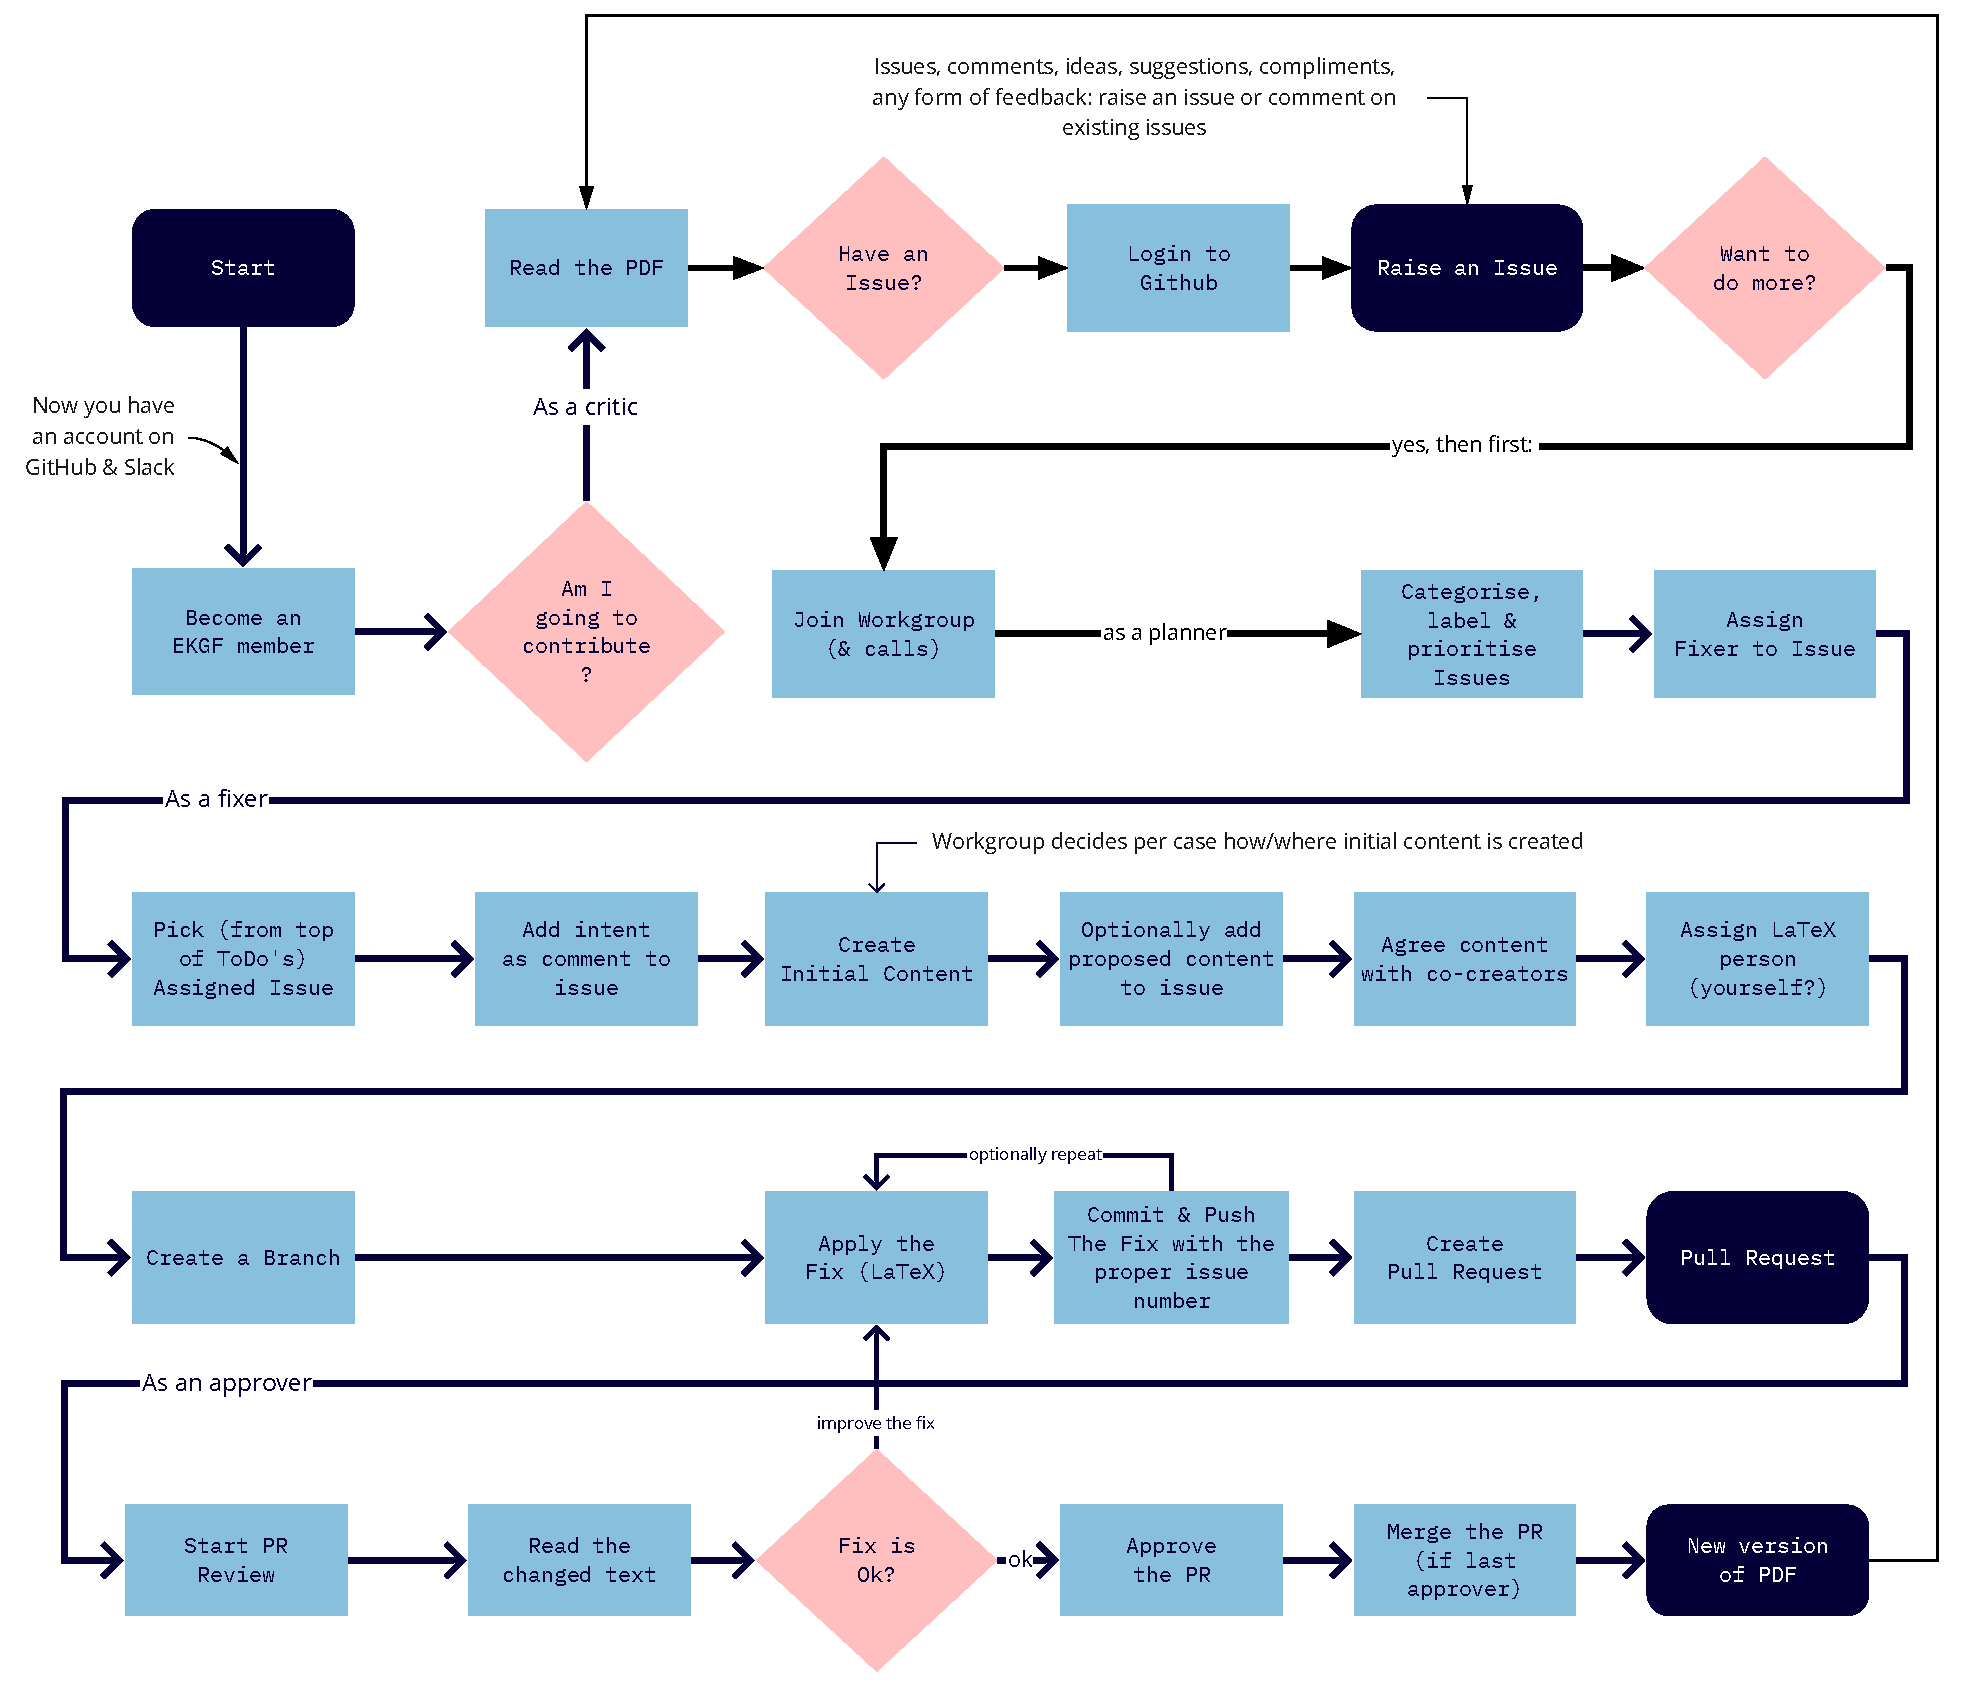
\includegraphics[width=\textwidth]{../images/ekgmm-process-diagram.pdf}
    \label{fig:ekg-mm-process-diagram}
\end{figure}

\section{Raise}
\label{sec:ekg-mm-process-raise}

\begin{tcolorbox}[colback=secondary!5,colframe=secondary!80,title=\textbf{User Stories}]
    \begin{itemize}[leftmargin=1em]
        \item As a \underline{critic}, I want to be able to \textbf{raise an issue}
    \end{itemize}
\end{tcolorbox}

Anyone who reads the produced content and has an issue with that content is a "critic".
Each critic should be able to raise that issue formally with minimal effort.

The audience of critics is hopefully very large, any reader of our content should
be able to add their comments somewhere.
We have to make it as easy as possible for them to do so. 

Unfortunately, the Issue Management function of private GitHub repositories--like
the \href{https://github.com/ekgf/ekg-mm}{EKGF/ekg-mm} repository--can only be
used by people who have a GitHub account (see \ref{subsec:ekg-mm-process-how-to-register}).

As someone in the role of a critic, you don’t have to deal with "\iindex{Agile}"
or "\iindex{Kanban}". 
The various workgroups/teams will plan for (see \ref{sec:ekg-mm-process-plan})
and process/fix (see \ref{sec:ekg-mm-process-fix}) your issues. 
You can always see the status of your issue by clicking on it and checking 
the right side of the screen where you see links to the "Assignee"
(the person who is going to work on your issue), the "Project"
(the workgroup that’s planning and tracking your issue) and the "Linked pull requests". 

\subsection{How to register?}
\label{subsec:ekg-mm-process-how-to-register}

We are asking every potential contributor, even someone who just wants to give us
some feedback (a "critic") to join the \gls{ekgf}.

The \gls{ekgf} supports free membership for individuals and corporate membership.

Email with \href{mailto:registration@ekgf.org}{registration@ekgf.org} to set it up,
if you plan to participate as a contributor to the \gls{ekgmm} then please also
supply your GitHub user id.

\subsubsection{How to create a GitHub \& Slack account?}

\paragraph{Slack}

If you already have a Slack account then join the \gls{ekgf} workspace here:
\url{https://ekgf.slack.com/}. Otherwise first create your Slack account here:
\url{https://slack.com/get-started#/create}.

\paragraph{GitHub}

Go to \url{https://github.com/join}.

Since you can associate multiple email addresses to your GitHub account we would
suggest to initially create it with your private email address which then becomes
your "primary email account" in GitHub.
You can add your business email address(es) to your GitHub account later.

Mail your GitHub account id (user id) to
\href{mailto:registration@ekgf.org}{registration@ekgf.org} so that we can add you
to to the access control list of the EKGF/ekg-mm repository.

\pagebreak
\subsection{How to read the content?}

If you’re interested in the latest version of the \gls{ekgmm} document,
which is published as a PDF document, then go to
\url{https://www.ekgf.org/maturitymodel} and download it from there.

\begin{wrapfigure}[18]{r}{0.5\textwidth}
    \vspace{-12pt}
    \begin{center}
        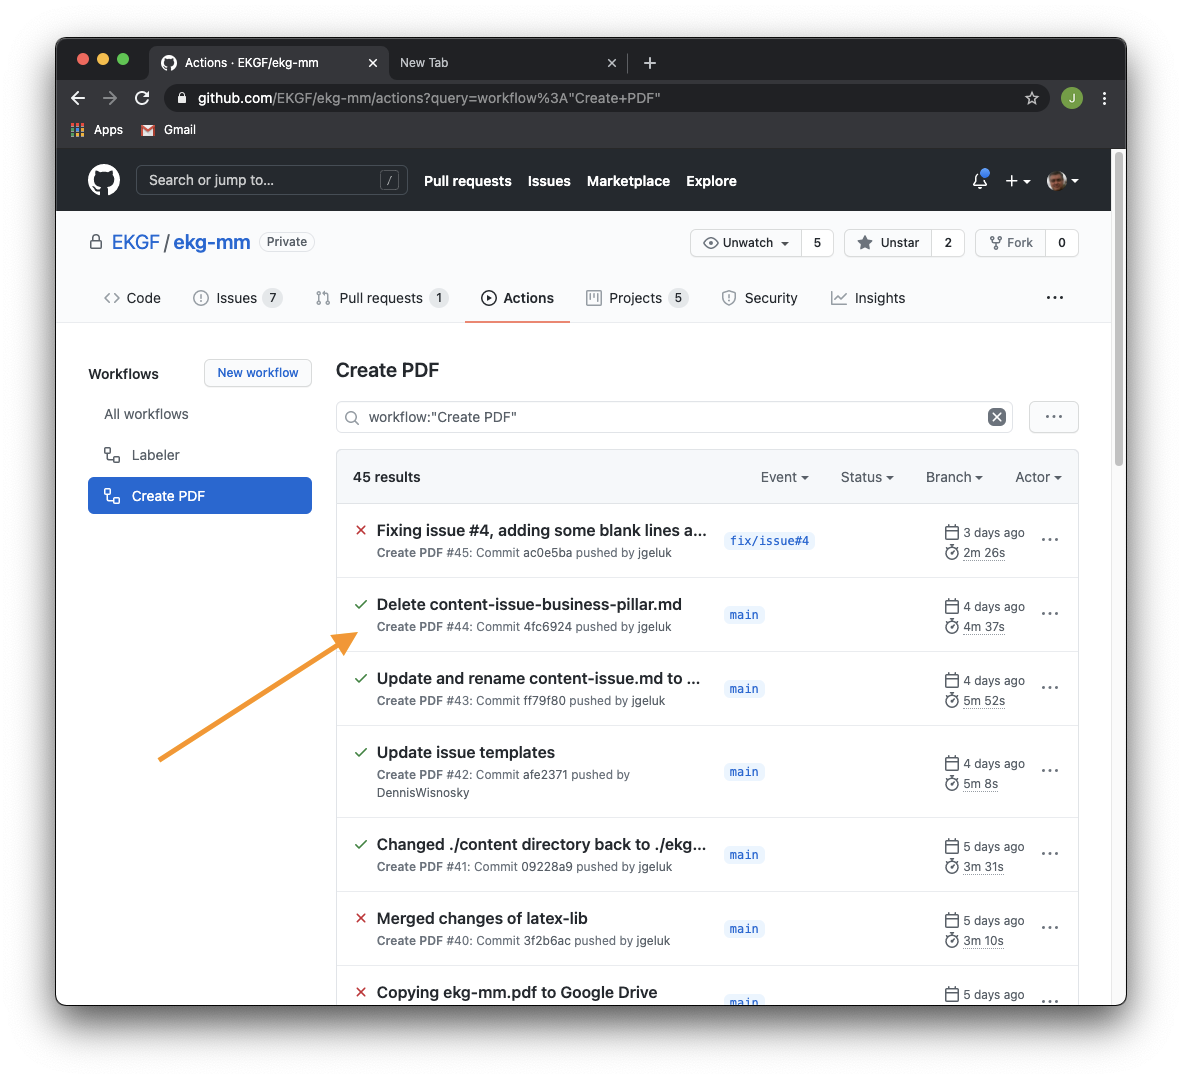
\includegraphics[width=0.50\textwidth]{../images/ekgmm-process-create-pdf-workflow.png}
    \end{center}
    \caption{Find your PDF}
    \label{fig:ekgmm-process-find-your-pdf}
\end{wrapfigure}

NOTE: At the moment we do not yet put the latest version of the generated 
PDF document on that webpage automatically so it can take a few days until 
\gls{ekgf} staff manually uploads the latest version to that webpage. 
We’re working on automating that last step of the "\gls{ci} Process".

\subsubsection{How to read specific versions of the PDF?}

For readers who would like to see “work in progress”, versions of the document 
that are being worked on in the various “branches” of the repository, 
there’s another way to get to the corresponding PDF document.

To see the latest content for any given branch, go to the "Actions" page 
on the GitHub website (\url{https://github.com/ekgf/ekg-mm/actions}) where you can 
find the \gls{ci}-build processes that create the PDF for each change 
(in git jargon that would be called "a push") in any branch.

In figure \ref{fig:ekgmm-process-find-your-pdf} you can see how you can 
find the latest successful run of the "Create PDF" workflow on the 
\texttt{main} branch (job \#44 in this case, the branch name is shown in blue).

%
% Wrap the figure on the left, give it 20 lines of vertical space and scale
% it down to half the text width
%
\begin{wrapfigure}[20]{l}{0.5\textwidth}
    \vspace{-12pt}
    \begin{center}
        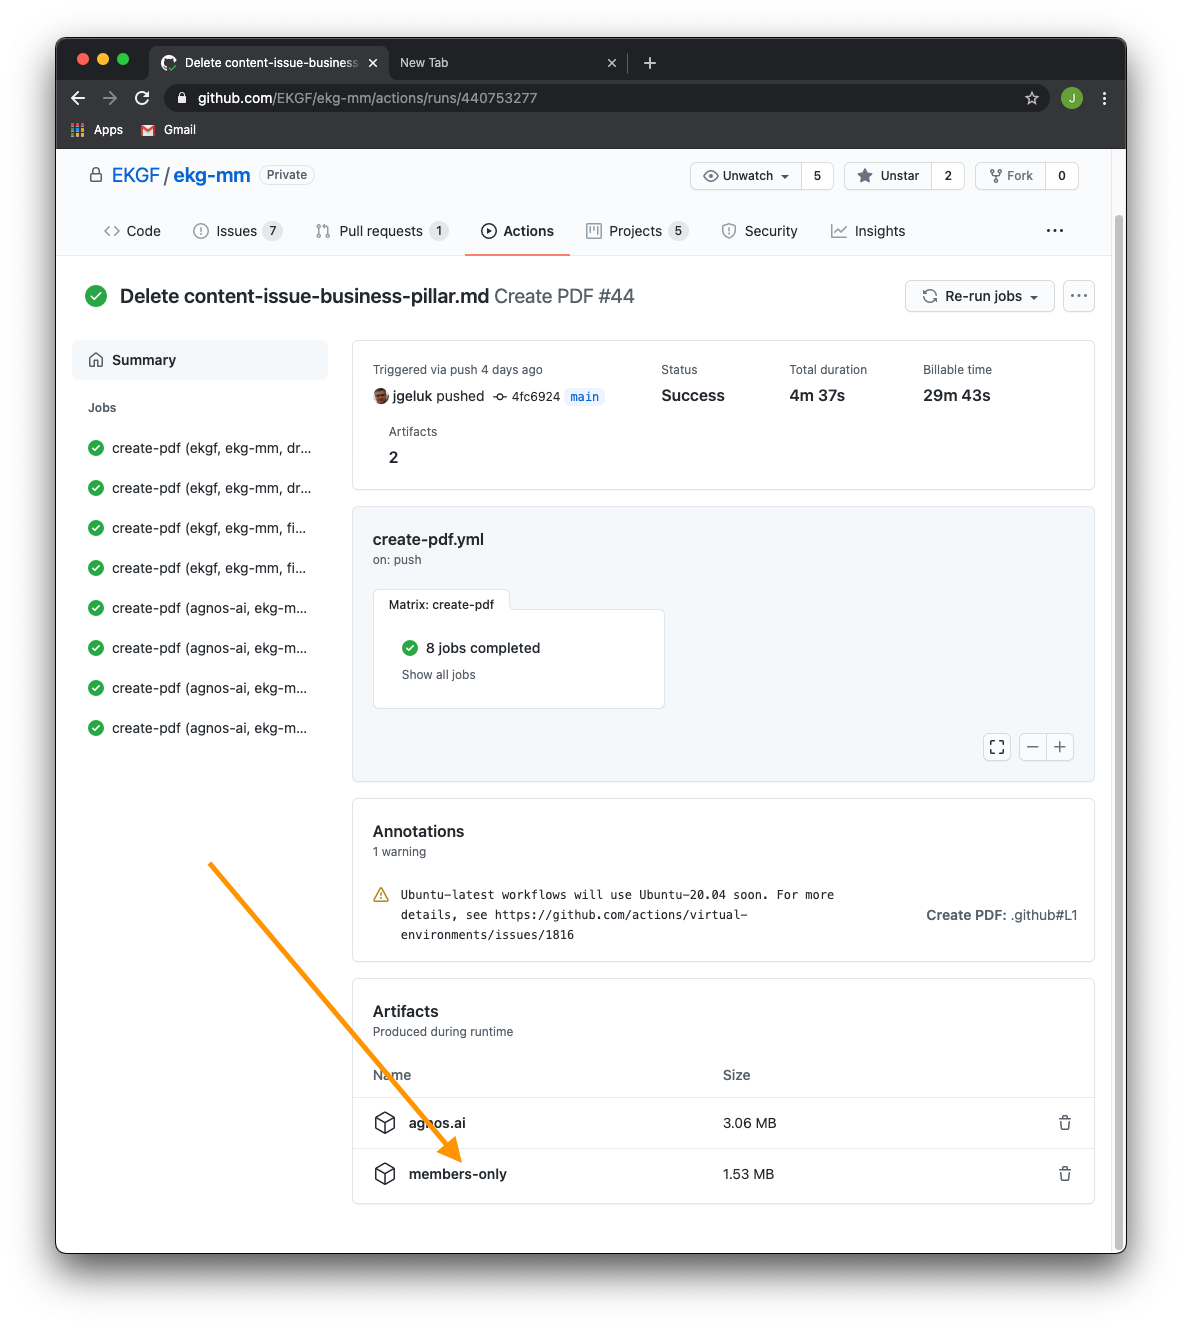
\includegraphics[width=0.50\textwidth]{../images/ekgmm-process-create-pdf-job.png}
    \end{center}
    \caption{The "Create PDF Job" page where you can find your PDF}
    \label{fig:ekgmm-process-create-pdf-job}
\end{wrapfigure}

When you then click on the name of that job, you will see the details of that job.
When the job ran successfully, "everything is green" as you can see in figure
\ref{fig:ekgmm-process-create-pdf-job}.
Scroll to the bottom where you will find the "members-only" link which gives you
a downloadable zip file with the "draft" and "final" version of the document.

\subsubsection{Document File Names}
\label{subsec:ekg-mm-process-document-file-names}

The ``create-pdf'' job as shown in figures \ref{fig:ekgmm-process-find-your-pdf}
and \ref{fig:ekgmm-process-create-pdf-job} generates two different versions of the PDF:

\begin{enumerate}[leftmargin=1.2em,font=\footnotesize]
    \item {\footnotesize\texttt{ekgf-ekg-mm-<version-number>.pdf}}
    \item {\footnotesize\texttt{ekgf-ekg-mm-draft-<version-number>.pdf}}
\end{enumerate}

The documents with "\texttt{draft}" in the file name have a wider right margin 
where all kinds of "notes" and "todo’s" can be shown (that are part of the content in git).
They can also contain new sections of the document that are not fully consistent yet.

\subsection{How to raise an issue?}
\label{subsec:ekg-mm-process-how-to-raise-an-issue}

While you’re reading the document, you may have comments, we hope you do.
Please raise as many "issues" as possible, any feedback is welcome.
An issue can be a question, a suggestion, a grammar issue, 
an issue with the consistency of the story, anything that comes to mind. 
If you decide to let us benefit from your feedback then please follow these steps:

\begin{itemize}
    \item Go to the main page where all issues are shown:
          \url{https://github.com/ekgf/ekg-mm/issues}
    \item Check if your issue is already raised by someone else, if so, 
          feel free to augment the discussion around that issue with your own concerns.
    \item If it clearly is a new issue, click the "New Issue" button.
    \item Give it a concise title and clear description and ideally:
    \begin{itemize}
        \item Copy paragraphs you don’t agree with into the issue
        \item Mention the paragraph number and version of the document (as shown on the front page) 
    \end{itemize}
    \item There is no need to specify values for any of the fields on
          the right side because the admin team will do that (but feel free to).
    \item Save by clicking the “Submit new issue” button
\end{itemize}

That’s it. Thank you very much. Every issue is a discussion page,
other people can respond to it and chip in. 
At some point, a workgroup will pick it up, assign it to their project board, 
plan for fixing it, etc. You will be notified of these changes 
automatically via GitHub email.

\section{Plan}
\label{sec:ekg-mm-process-plan}

\begin{tcolorbox}[colback=secondary!5,colframe=secondary!80,title=\textbf{User Stories}]
    \begin{itemize}[leftmargin=1em]
        \item As a \underline{planner}, I want to be able to \textbf{plan issues}
    \end{itemize}
\end{tcolorbox}

Work on the \gls{ekgmm} is divided among workgroups that each take on an MM pillar
or horizontal slice of the MM. 
Workgroups are self-managed teams. 
The workgroups meet on a regular schedule. 
Any method that the team agrees to use to plan and to document issues during 
working sessions is ok. 
But, the official content of the MM is contained in the GitHub repository 
that is managed using the GitHub Kanban with review and automation process.

Here are some useful links. 

\begin{itemize}
    \item \href{https://www.atlassian.com/agile/kanban}{Kanban - A brief introduction}
    \item \href{https://www.atlassian.com/agile/kanban/boards}{What is a Kanban Board?}
\end{itemize}

The idea is very simple though, we use the GitHub Projects facility. 
Currently, we have a project for each pillar and a general project. 
Here’s the main page for \gls{ekgmm} GitHub Projects:

\begin{center}
    \url{https://github.com/ekgf/ekg-mm/projects}
\end{center}

What you see is a list of "project boards" where each project board 
is owned by a workgroup in the entire Kanban process. 
This begins with planning. 

The planning process consists of various tasks:

\begin{itemize}
    \item Find open issues that are relevant to the workgroup in the list of issues:
    \begin{itemize}
        \item Here is a link: \href{https://github.com/EKGF/ekg-mm/issues?q=is%3Aissue+is%3Aopen+no%3Aproject}
              {open issues that have not yet been assigned to a project board}
    \end{itemize}
    \item Link each issue that should be done by the workgroup to its
          corresponding project board.
          It will then appear at the bottom of the “To Do” column of that board.
    \item Decide priority (see \ref{subsec:ekg-mm-process-to-do-column}).
    \item Assign issues to members of the workgroup.
    \begin{itemize}
        \item By linking the issue to one or more assignees
              (open the issue by clicking on it and select the assignee at
              the top right corner)
    \end{itemize}
    \item Follow the progress of issues as they go from left to right via the columns on the board.
\end{itemize}

\subsection{"To Do" Column}
\label{subsec:ekg-mm-process-to-do-column}

As soon as an issue has been assigned to a given project, 
it will show up at the bottom of the \iindex{To-Do Column}. 
That To-Do Column can be seen as "the backlog"\index{Backlog} 
for that project (and for the workgroup that owns that project).

Issues can be dragged and dropped within the To-Do Column. 
Issues at the top have the highest priority. 
Anyone in the workgroup can pick up issues assigned to 
them and start "fixing" them (which means resolving them), 
see \secref{sec:ekg-mm-process-fix}.

\subsection{"In progress" Column}\index{In Progress Column}

Pull Requests and Issues\footnote{Issues are sometimes also 
called “Cards” in Kanban terminology and in the Github project 
user interface.
Besides that you can also add “Notes” to the project board.} 
show up in this column automatically as soon as someone is 
actually working on the issue, see \secref{sec:ekg-mm-process-fix}.

This means that as soon as a fixer "pushes" one or more "commits" 
to the GitHub repository that this will be seen as progress 
and show up accordingly on the project board.

\subsection{"Review in progress" Column}

Once the fixer has created their \gls{pr}, they can ask 
for a review of the \gls{pr} by selecting two or more reviewers. 
See \secref{sec:ekg-mm-process-approve} for information about how to do a review.

\subsection{"Reviewer approved" Column}

Once all reviewers have approved the \gls{pr}, 
the last reviewer can then merge the \gls{pr} into the main branch. 
By the way, a reviewer can also reject a change or ask for 
changes to be applied before approving the \gls{pr}. 

The fixer then has to then apply new changes and commit 
them to the same branch and push those changes to GitHub. 
The \gls{pr} page will then be updated automatically and a subsequent 
review process can then commence.
As said above, once all approvals are given, 
the changes can then be merged by the final reviewer 
into the main branch which will trigger the final build 
workflow on GitHub creating the publishable content as 
PDF (and eventually also as HTML).

\subsection{"Done" Column}
\label{subsec:ekg-mm-process-done-column}

When the merge of the \gls{pr} is done the issue will move to 
the Done column. 

For each \gls{pr} there is an underlying git branch which 
will be automatically deleted by GitHub once the \gls{pr} 
has been merged into the main branch.

\pagebreak
\section{Fix}
\label{sec:ekg-mm-process-fix}

\begin{tcolorbox}[colback=secondary!5,colframe=secondary!80,title=\textbf{User Stories}]
    \begin{itemize}[leftmargin=1em]
        \item As a \underline{fixer}, I want to be able to \textbf{fix issues}
        \item As a \underline{fixer}, I want to be able to \textbf{create a pull request}
    \end{itemize}
\end{tcolorbox}

The term "fixer"\index{Fixer} is our own term, they’re usually called "developer" but 
we don’t consider someone who works on \gls{ekgmm} content to be a developer necessarily.
In the GitHub user interface, they show up as "contributors"\index{Contributor}.
Anyone who actually changes things in the repository will be registered by GitHub as 
a contributor to that repository\footnote{The GitHub userids and names of all 
contributors will be listed in the final output \gls{ekgmm} document.}.

There are many different ways to change the content of the repository. 
There are roughly two methods though:

\begin{enumerate}[label=(\Alph*)]
    \item Change content without making a "clone" of the repository by editing content on the GitHub site itself.
    \item Make a so-called "git clone" of the repository to your own workstation and use any appropriate editor to add or change things.
\end{enumerate}

%
% Wrap the figure on the left, give it 20 lines of vertical space and scale
% it down to half the text width
%
\begin{wrapfigure}[16]{r}{0.5\textwidth}
    \vspace{-12pt}
    \begin{center}
        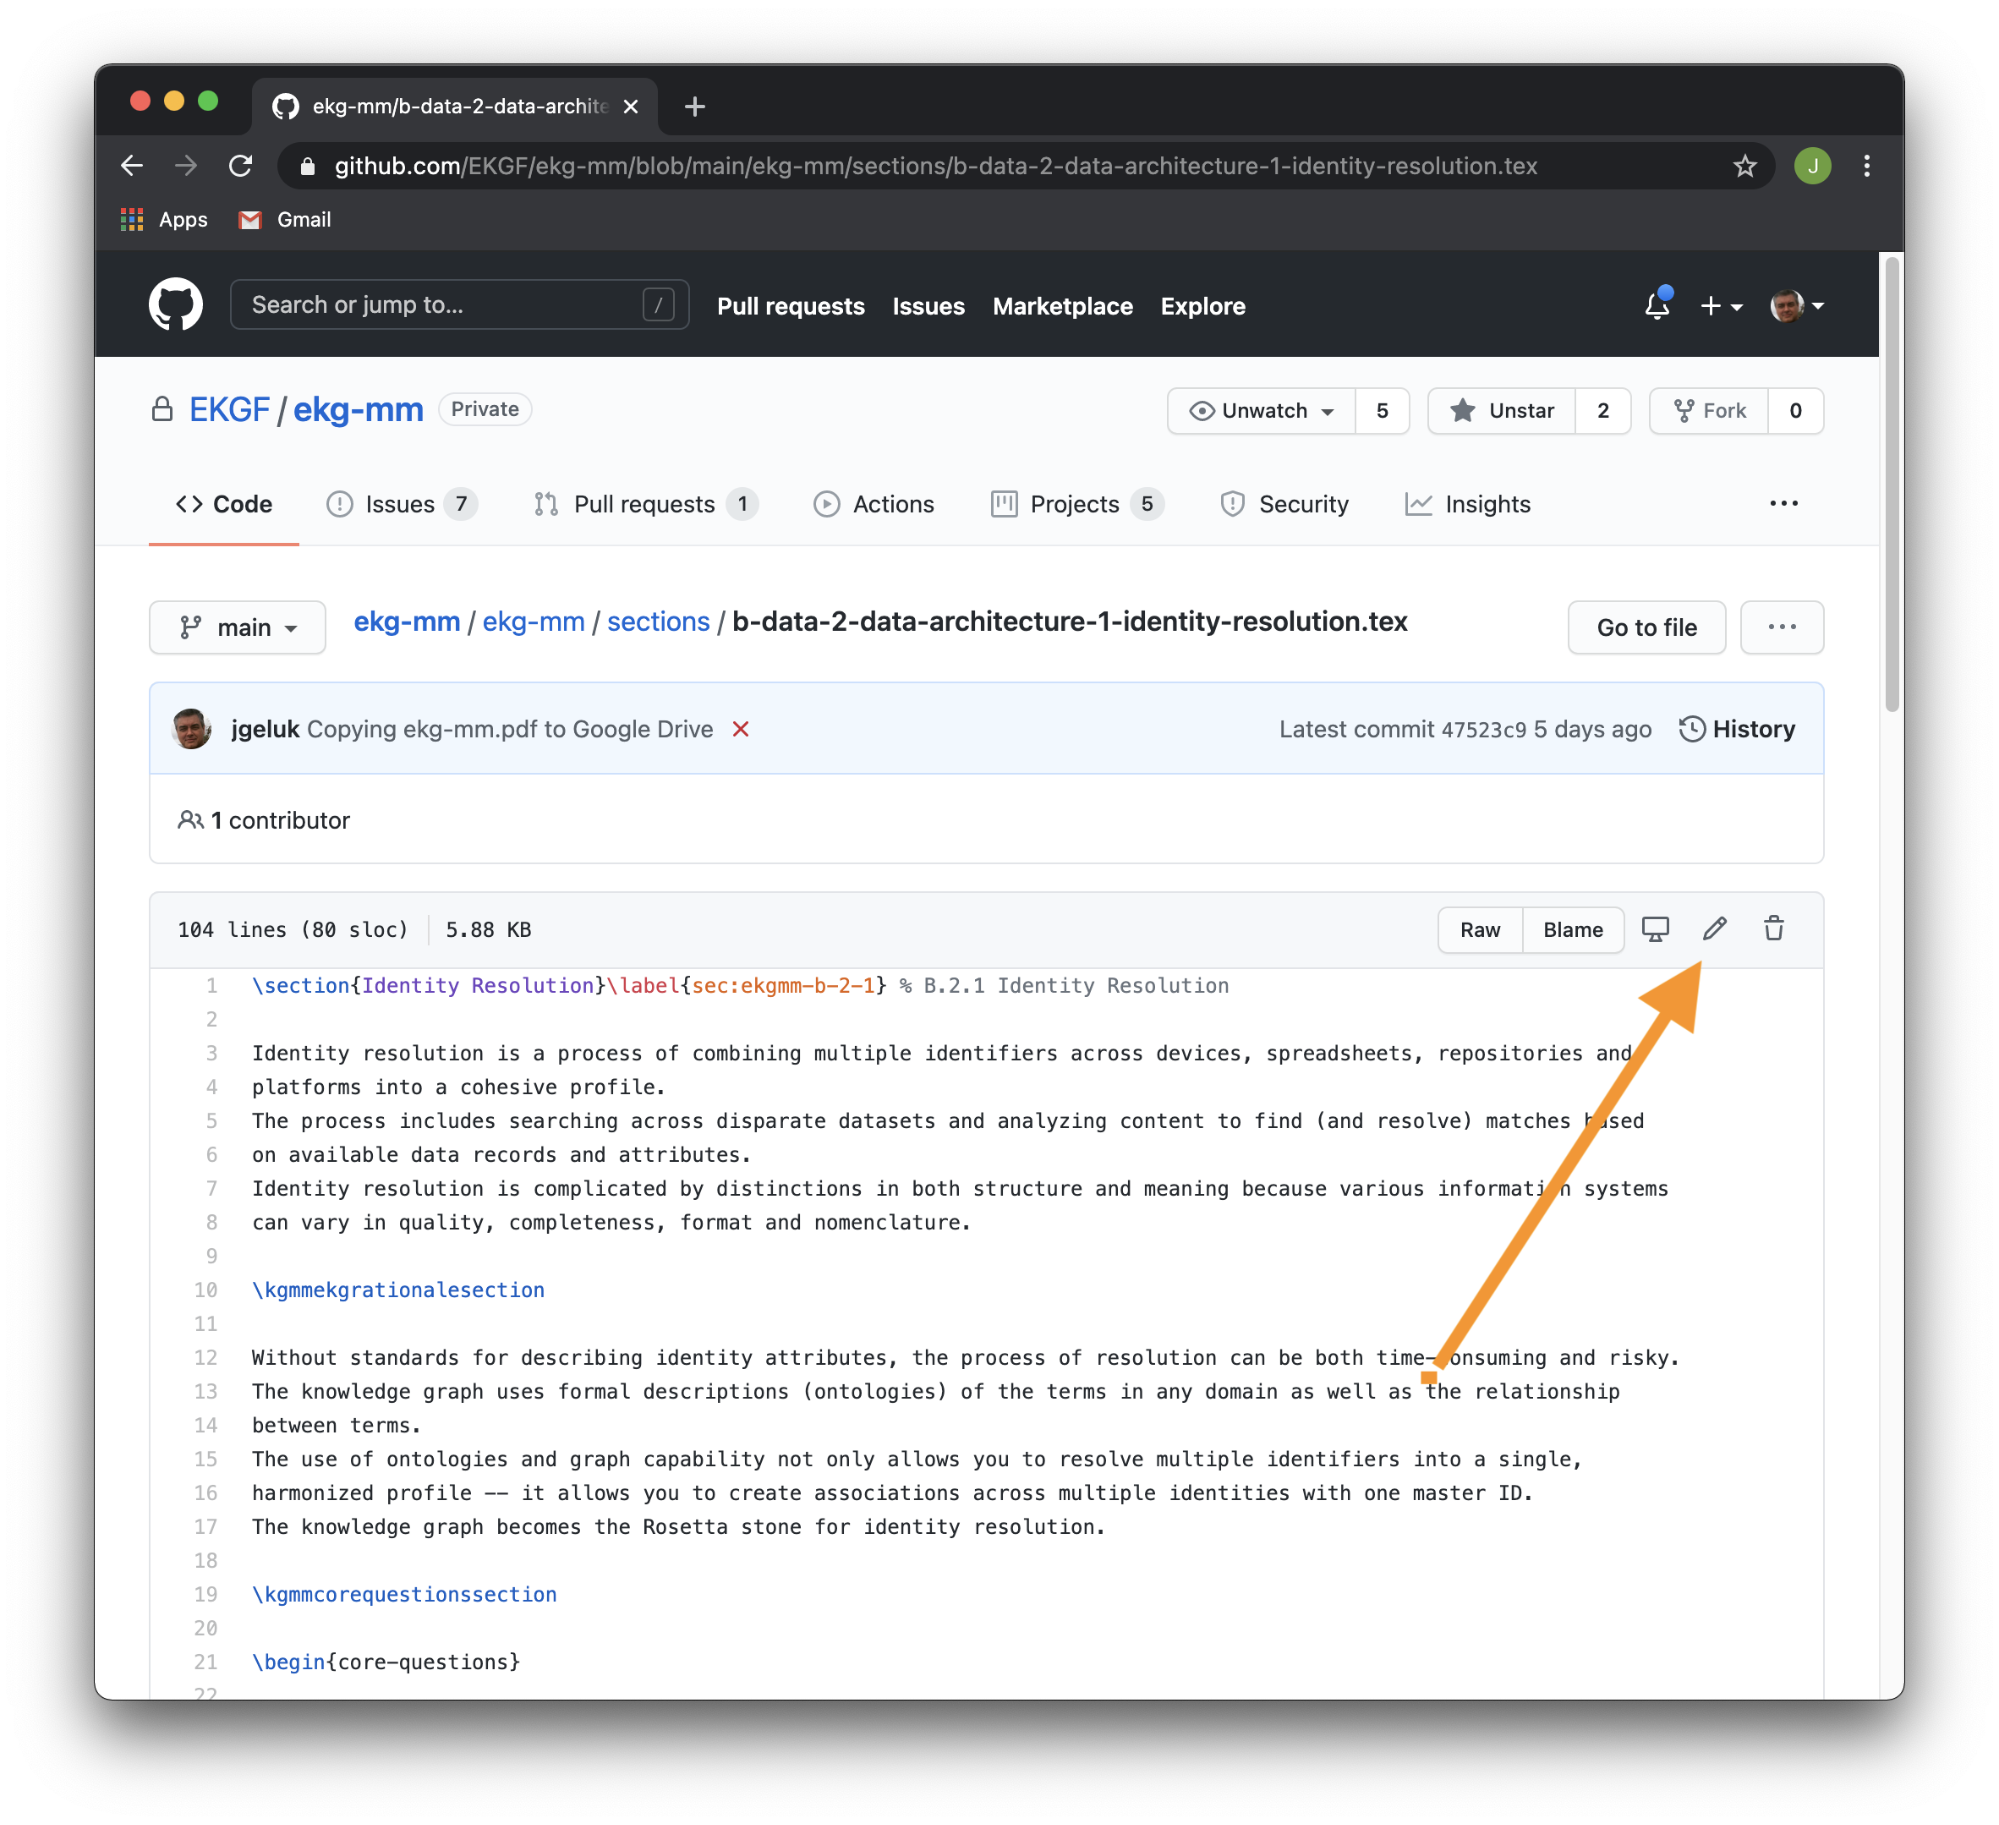
\includegraphics[width=0.50\textwidth]{../images/ekgmm-process-edit-content.png}
    \end{center}
    \caption{Where to find the edit button}
    \label{fig:ekgmm-process-edit-content}
\end{wrapfigure}

Both methods require:

\begin{itemize}
    \item "creating a branch" (See \ref{subsec:ekg-mm-process-how-to-make-a-branch})
    \item "committing a change" (See \ref{subsec:ekg-mm-process-how-to-commit})
    \item "creating a pull request" (See \ref{subsec:ekg-mm-process-how-to-create-a-pull-request})
\end{itemize}

We will now describe how each of these three tasks can be done.

\subsection{How to start editing in GitHub?}

This is "Method A" as described above.
First find the content file that you want to edit.
All content is under the content root directory \texttt{/ekg-mm}.

The arrow in figure \ref{fig:ekgmm-process-edit-content} above shows the
location of the "edit button" (ignore the other buttons). 
Click that button and change any content. 
All content is written in a "language" called \iindex{LaTeX} which is
a markup language for professional content (used for books and Ph.D. 
thesis and the like).
As long as you keep the LaTeX commands (aka macros) in place (they 
start with a backslash) things will be fine, just type away. 
Unless you know LaTeX (a little) then you can add whatever works.

Then it’s time to save the changes, choose a good title for your 
change, and include the issue number (for instance \texttt{\#123})
prefixed with a hash.
This title is the so-called "commit message" and is described in 
more detail in \subsecref{subsec:ekg-mm-process-how-to-commit}.

\subsection{How to make a branch?}
\label{subsec:ekg-mm-process-how-to-make-a-branch}

When editing straight on the GitHub site as described in the previous 
section, you have to save your work "as a commit" with a title that 
contains the issue number (which will be picked up by the project board). 
But you then also have to create a branch which shows up right under 
the title and description. 

Choose a branch name that explains what it is about. 
In some cases that would be all there is to it but in most cases you 
have multiple edits in multiple files for one given issue. 
So in those cases you would have to make sure to always refer to 
the right branch name where the branch name must include the 
issue number itself. 
For instance, for issue \texttt{\#123} the branch name would 
be \texttt{issue-123}.

\subsection{How to commit a change?}
\label{subsec:ekg-mm-process-how-to-commit}

%
% Wrap the figure on the left, give it 20 lines of vertical space and scale
% it down to half the text width
%
\begin{wrapfigure}[20]{l}{0.5\textwidth}
    \vspace{-12pt}
    \begin{center}
        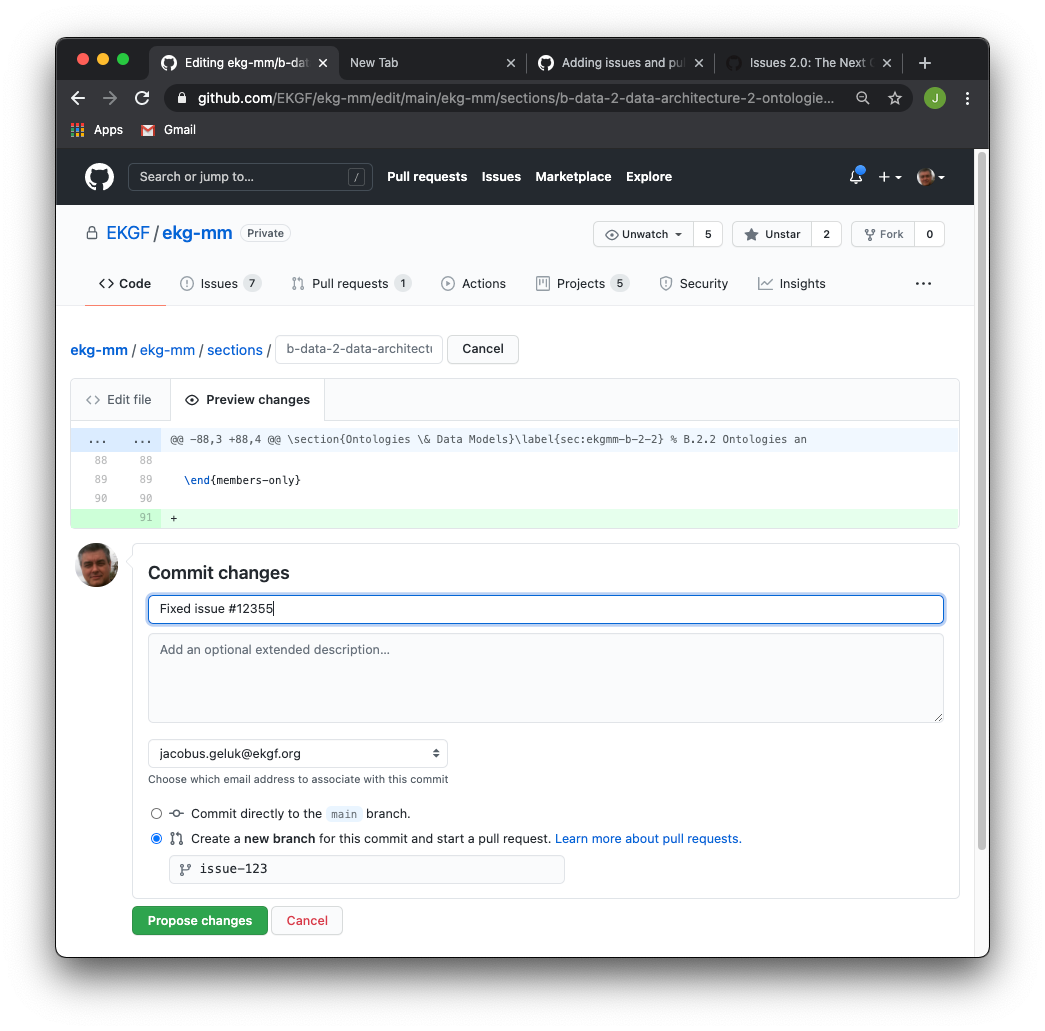
\includegraphics[width=0.50\textwidth]{../images/ekgmm-process-commit-changes.png}
    \end{center}
    \caption{Committing changes}
    \label{fig:ekgmm-process-commit-changes}
\end{wrapfigure}

There are many different ways to create a commit on a branch in a 
git repository. It’s up to the "fixer" (usually called "developer"
in most git documentation on the Internet) to decide which
tooling they use.
One way to do this is to just use the Github website itself but you
could also create a so-called "clone" of the git repository on your 
local machine and use the standard git utility to create a commit or 
use an advanced editor like Visual Studio Code that has built-in 
git support and a LaTeX plugin. 
It goes too far to document all the various different ways to do this 
in the context of this document.
What’s important to know is that, as a fixer, you should always include
the issue number in the title of the commit. 
For example, if you edit a content page and then commit that change, 
you have to make sure that these two things are done before clicking 
the "Propose Changes" button as shown in figure \ref{fig:ekgmm-process-commit-changes}.

Use a title for your commit that includes the issue number, 
prefixed by \texttt{\#}, for example, \texttt{\#123} for issue 123.
Use a branch name that includes the issue number (no hash as a prefix).

The \texttt{\#123} in the title will trigger GitHub to move the
corresponding issue from the "To Do" column to the "In Progress" column.
Do not use "Fixed \texttt{\#123}" or “Close \texttt{\#123}” because that 
will actually close the issue.

Once you have done your first commit to a given branch, you’re ready to
create a \gls{pr}. 
Many people wait with creating a \gls{pr} until their last commit is pushed
(one issue can involve many commits involving many files but they all 
go to the same branch) but we recommend creating your \gls{pr} as soon as possible, 
after the first commit, because that gives everyone an easier insight 
in the progress. Not everyone is up for that, “exposing” their 
first draft changes to others, but it’s generally seen as 
good practice to do so. 
You can mark your \gls{pr} as “Draft” via the GitHub user interface so that 
everyone knows that it is “work in progress”.

\subsection{How to create a pull request?}
\label{subsec:ekg-mm-process-how-to-create-a-pull-request}

Assuming that you added some changes to a branch, in GitHub parlance: 
"pushed some commits to a branch", you can also create a \gls{pr}. 
A \gls{pr} can be seen as a "request approval to change"-form. 
It needs two branches: the branch that you want to change (that would 
usually be the main branch) and the branch that contains the new version 
with the proposed changes. 
GitHub automatically calculates the difference between those two branches
and shows those differences on the \gls{pr}-form.

There are several different places in the GitHub user interface where you 
can start creating a \gls{pr} but the most basic one shows up at the branches 
page which shows all branches of the repository:

\begin{center}
    \url{https://github.com/ekgf/ekg-mm/branches}
\end{center}

On the right side of the table showing all the branches you either see an 
existing \gls{pr} for the given branch or a button:

\begin{center}
    
\includegraphics[scale=0.5]{../images/ekgmm-process-pr-button.png}
\end{center}

It’s easy from there. 
Give your \gls{pr} a good title (that title goes into the "changelog" so be 
specific) and a description and click the Create Pull Request button. 
Job done. A planner in the workgroup will take it from there, 
assign reviewers, link it to a project board etc.

\section{Approve}
\label{sec:ekg-mm-process-approve}

\begin{tcolorbox}[colback=secondary!5,colframe=secondary!80,title=\textbf{User Stories}]
    \begin{itemize}[leftmargin=1em]
        \item As a \underline{reviewer}, I want to be able to \textbf{approve pull requests}
    \end{itemize}
\end{tcolorbox}

TODO

\end{document}
